%!TEX root=main.tex
\section{背景}
\label{clicknp:sec:background}

\subsection{软件虚拟网络与网络功能的性能挑战}


虚拟网络通常用虚拟交换机软件实现,如 Open vSwitch \cite{pfaff2015design}。
为了提高虚拟网络的性能,并满足可编程性要求,云服务商重新设计了软件虚拟交换机。
通过利用 DPDK \cite{dpdk} 等高速网络处理包技术,并使用轮询模式运行 CPU 核,可以绕过 OS 网络协议栈来显著降低数据包处理成本。
%SoftNIC \cite{han2015softnic} 提出用软件实现网卡中固化的功能以提高灵活性。
但是,即使是不做任何处理的简单网络数据包转发,每个 CPU 核每秒也只能处理 10 M 至 20 M 个数据包 \cite{martins2014clickos,netbricks},对于 60 M 个数据包每秒的 40 Gbps 线速,仍然需要 3 至 6 个 CPU 核。

传统的网络功能由部署在数据中心特定位置的专用设备实现,如 F5 负载均衡器 \cite{f5-load-balancer}。这些专用网络功能设备不仅价格高昂,也不够灵活,不足以支持云服务中的多租户。
为了支持灵活的网络功能,云服务商还部署了软件实现的虚拟网络功能。例如,Ananta \cite {ananta} 是一个部署在微软数据中心的软件负载均衡器,用于提供云规模的负载均衡服务。
为了在一台服务器上支持多种网络功能,RouteBricks \cite {routebricks}、xOMB \cite{anderson2012xomb} 和 COMB \cite{comb} 采用 Click 模块化路由器 \cite{kohler2000click} 的编程模型,把每个网络功能实现成一个 C++ 的类,让每个数据包在一个 CPU 核上依次被各个网络功能处理,即所谓 ``运行到结束(run-to-completion)'' 模型。
这些工作表明,在实际网络功能下,基于多核 x86 CPU 的每台服务器转发数据包的速度可达 10 Gbps,并且可以通过多核和搭建更多网络节点的集群来扩展容量。
为了实现网络功能之间的隔离,NetVM \cite{hwang2015netvm}、ClickOS \cite{martins2014clickos}、HyperSwitch \cite{ram2013hyper}、mSwitch \cite{eisenbud2016maglev} 等工作把每个网络功能放在一个(轻量级)虚拟机里,并让虚拟交换机把数据包依次分发给这些虚拟机处理,即所谓 ``流水线'' 模型。
流水线模型中,数据包在多核之间反复传递,开销较高。
NetBricks \cite{netbricks} 回到了 ``运行到结束'' 模型,但用高级语言实现网络功能,并在编译器和运行框架的层面上保证网络功能之间的隔离性。
NFP \cite{sun2017nfp} 利用多个并行的网络功能流水线提高数据包处理的性能。

虽然软件实现的虚拟交换机和网络功能可以使用更多数量的 CPU 核和更大的网络节点集群来支持更高的性能,但这样做会增加相当大的资产和运营成本 \cite {ananta,duet}。
云服务商在 IaaS 业务中的盈利能力是客户为虚拟机支付的价格与托管虚拟机的成本之间的差异。
由于每台服务器的资产和运营成本在上架部署时就已基本确定,因此降低托管虚拟机成本的最佳方法是在每台计算节点服务器上打包更多的客户虚拟机,并减少网络和存储节点的服务器数量。
目前,物理 CPU 核(2 个超线程,即 2 个 vCPU)的售价为 0.1 美元/小时左右,亦即最大潜在收入约为 900 美元/年 \cite{smartnic}。
在数据中心,服务器通常服役 3 到 5 年,因此一个物理 CPU 核在服务器生命周期内的售价最高可达 4500 美元 \cite{smartnic}。
即使考虑到总有一部分 CPU 核没有被售出,并且云经常为大客户提供折扣,与专用硬件相比,即使专门分配一个物理 CPU 核用于虚拟网络也是相当昂贵的。

为了加速虚拟网络和网络功能,以前的工作已经提出使用 GPU \cite {packetshader},网络处理器(Network Processor,NP) \cite {cavium,netronome} 和硬件网络交换机 \cite {duet}。
GPU 早期主要用于图形处理,近年来扩展到具有海量数据并行性的其他应用程序。
PacketShader \cite {packetshader} 表明使用 GPU 可以实现 40Gbps 的分组交换速度。
GPU 适合批量操作,但是,批量操作会导致高延迟。
例如,PacketShader \cite {packetshader} 报告的转发延迟约为 $200 \mu{}s$,比 \name{} 高两个数量级。
如第 \ref{smartnic-fpga} 节讨论的,与GPU相比,FPGA可以充分利用流水线并行、数据并行和请求并行,实现低延迟、高吞吐量的数据包处理。
网络处理器专门用于处理网络流量并且具有许多硬连线(hard-wired)的网络加速器。
NP-Click \cite{shah2004np} 在网络处理器上实现了 Click 编程框架。
Click 模块化路由器 \cite{kohler2000click} 提出的第二年,NP-Click \cite{shah2004np} 就在网络处理器上实现了 Click 编程框架。
如第 \ref{smartnic-np} 节讨论的,网络处理器的主要问题是单流(single flow)吞吐量受单核性能局限。
如第 \ref{background:sec:network-function} 节讨论的,硬件网络交换机的主要问题是灵活性和查找表容量不足 \cite {duet}。

如第 \ref{smartnic-fpga} 节讨论的,使用 FPGA 来做网络功能处理存在一系列挑战,本文关注利用大规模并行性和编程工具链两个方面。
与CPU或GPU相比,FPGA通常具有更低的时钟频率和更小的存储器带宽。
例如,FPGA的典型时钟频率约为200MHz,比CPU慢一个数量级(2至3~GHz)。
同样,FPGA的单块存储器或外部DRAM的带宽通常为2至10~GBps,而Intel Xeon CPU的DRAM带宽约为60~GBps,GPU的GDDR5或HBM带宽可高达数百 GBps。
但是,CPU或GPU只有有限的内核,这限制了并行性。 FPGA内置了大量的并行性。
现代FPGA可能拥有数百万个LE,数百个K位寄存器,数十个M位BRAM和数千个DSP模块。从理论上讲,它们中的每一个都可以并行工作。
因此,FPGA芯片内部可能会同时运行数千个并行的``\textit {核}''。
虽然单个BRAM的带宽可能有限,但如果并行访问数千个BRAM,则总内存带宽可达数TBps!
因此,为了实现高性能,程序员必须充分利用这种大规模的并行性。

传统上,FPGA使用诸如Verilog和VHDL之类的硬件描述语言进行编程。
这些语言水平太低,难以学习,编程也很复杂。
因此,大型软件程序员社区已经远离FPGA多年了~\cite {bacon2013fpga}。
为了简化 FPGA 编程,工业界和学术界开发了许多高级综合工具和系统,旨在将高级语言(主要是C)的程序转换为硬件描述语言。
但是,正如下一小节将讨论的,它们都不适合网络功能处理,这是本工作的重点。

\subsection{基于 FPGA 的网络功能编程}

本章的目标是利用FPGA加速构建一个多功能,高性能的网络功能平台。这样的平台应满足以下要求。

\textbf {灵活性。} 平台应该\textit {完全使用高级语言编程。}
开发人员应当能使用高级抽象和熟悉的工具编程,就像在多核处理器上编程一样。
这是使大多数软件程序员可以使用FPGA的必要条件。

\textbf {模块化。} 网络功能平台应该支持\textit {模块化架构}进行数据包处理。以前关于虚拟化网络功能的经验表明,正确的模块化架构可以很好地捕获数据包处理中的许多常见功能~\cite {kohler2000click,martins2014clickos},使它们易于在各种网络功能中重用。

\textbf {高性能、低延迟。} 数据中心的网络功能应该以40 / 100~Gbps的线路速率处理大量数据包,具有超低延迟。以前的工作已经显示~\cite {rollback-mb},即使网络功能添加的几百微秒的延迟也会对服务体验产生负面影响。

\textbf {支持 CPU/FPGA 联合数据包处理。} FPGA 不是万能药。
正如第 \ref{smartnic-fpga} 节所讨论的,并非所有任务都适用于FPGA。
FPGA 中也无法容纳较大的逻辑。
因此,应该支持CPU和FPGA之间的细粒度处理分离。这需要CPU和FPGA之间的高性能通信。


FPGA 长期被用于实现网络路由器和交换机。
NetFPGA \cite{lockwood2007netfpga} 提出了一个在 FPGA 上实现路由器的开放硬件平台。
近年来,FPGA 也被用于加速网络功能 \cite {rubow2010chimpp,lavasani2012compiling}。
早在 Click 模块化路由器 \cite{kohler2000click} 编程框架被提出的第二年,Xilinx 就提出了用 FPGA 实现 Click 的 Cliff \cite{kulkarni2004mapping},需要硬件开发人员使用硬件描述语言把一个 Click 元件实现为一个硬件模块。
此后,CUSP \cite{schelle2005cusp} 和 Chimpp \cite {rubow2010chimpp} 提出了一系列改进,简化了硬件模块的互连,提高了软硬件协同处理、软件仿真的能力。
然而,上述工作使用 Verilog、VHDL 等硬件描述语言编程 FPGA。众所周知,硬件描述语言难以调试、编写和修改,给软件人员使用 FPGA 带来了很大挑战。

为了提高 FPGA 的开发效率,FPGA厂商提供了高层次综合(HLS)工具~\cite{vivado,intel-hls},可以把受限的 C 代码编译成硬件模块。但这些工具只是硬件开发工具链的补充,程序员仍然需要手动将从C语言生成的硬件模块插入到硬件描述语言的项目中,且 FPGA 与主机 CPU 之间的通信也需要自行处理。学术界和工业界提出了 Bluespec \cite{bluespec}、Lime \cite{auerbach2010lime} 和 Chisel \cite{bachrach2012chisel} 等高效硬件开发语言 \cite{bacon2013fpga,singh2011implementing,wester2015transformation},但它们需要开发者具有足够的硬件设计知识。Gorilla \cite {lavasani2012compiling} 为 FPGA 上的数据包交换提出了一种领域特定的高级语言。高层次综合工具和高效硬件开发语言可以提高硬件开发人员的工作效率,但仍然不足以让软件开发人员使用 FPGA。

Click2NetFPGA~\cite {Click2NetFPGA} 利用高层次综合工具,直接将 Click 模块化路由器 \cite {kohler2000click} 的 C++ 代码编译到 FPGA 来提供模块化架构。
然而,Click2NetFPGA 的性能的系统设计存在若干瓶颈(例如,内存和数据包 I/O),它们也没有优化代码以确保完全流水线处理,因此比本文达到的性能低两个数量级。
此外,Click2NetFPGA 不支持 FPGA / CPU 联合处理,因此无法在数据平面运行时更新配置或读取状态。

近年来,为了让软件开发人员使用FPGA,FPGA厂商提出了基于OpenCL的编程工具链~\cite{aoc,sdaccel},提供了类似GPU的编程模型,如图 \ref{intro:fig:opencl} 所示。软件开发人员可以把用OpenCL语言编写的核(kernel)卸载到FPGA上。


\begin{figure}[htbp]
	\centering
	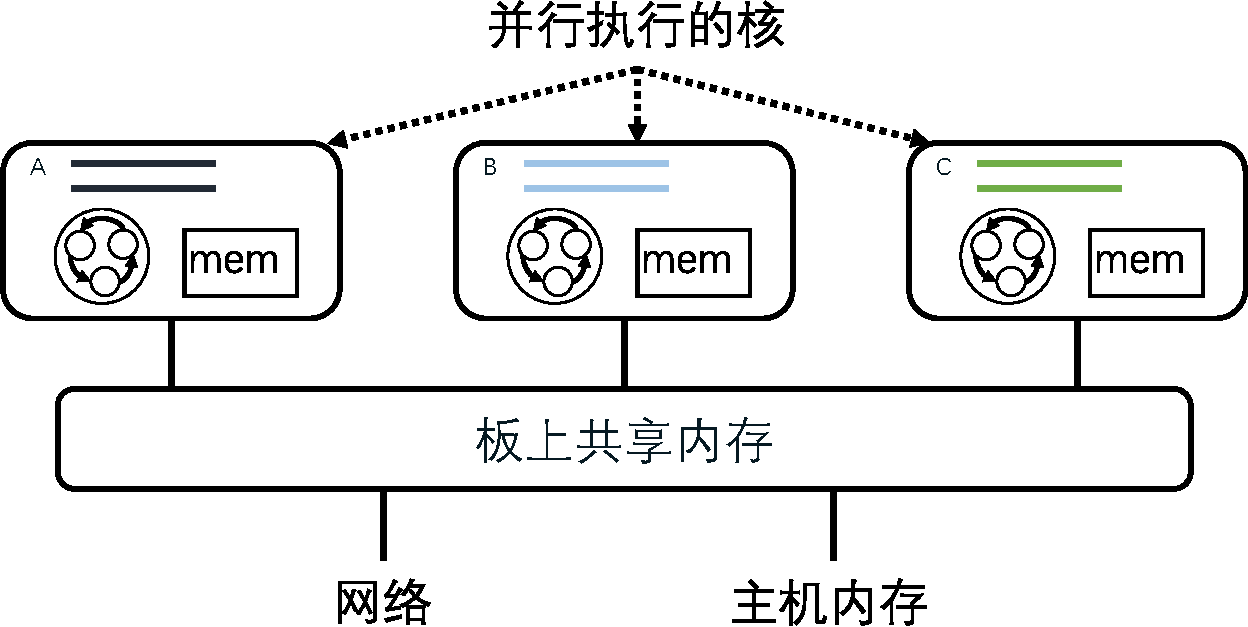
\includegraphics[width=0.7\textwidth]{../figures/opencl.pdf}
	\caption{OpenCL 核之间以及核与网络、主机的通信方式:共享内存。}
	\label{intro:fig:opencl}
\end{figure}


但是,这种方法中多个并行执行的核间需要通过板上共享内存进行通信,而FPGA上的DRAM吞吐量和延迟都不理想,共享内存还会成为通信瓶颈。
其次,FPGA与CPU之间的通信模型是类似GPU的批处理模型,主机程序和FPGA内核之间的通信必须始终通过板载DDR内存。这使得处理延迟较高(约1毫秒),不适用于需要微秒级延迟的网络数据包处理。
第三,OpenCL内核函数需要宿主机上的软件程序显式调用。
在内核终止之前,主机程序无法控制内核行为,例如设置新参数,也不能读取任何内核状态。
但是网络功能面临着连续的数据包流,应该始终在运行。
第四,OpenCL不支持CPU和FPGA之间的联合数据包处理,CPU上的数据包处理只能在 OpenCL 框架以外进行。

由于网络数据包处理是流式处理,并行执行的核之间应当通过管道(FIFO)而非共享内存来通信,如图 \ref{intro:fig:element_conn} 所示。FPGA 内的处理逻辑与网络和主机之间也应当通过管道来通信。

\begin{figure}[htbp]
	\centering
	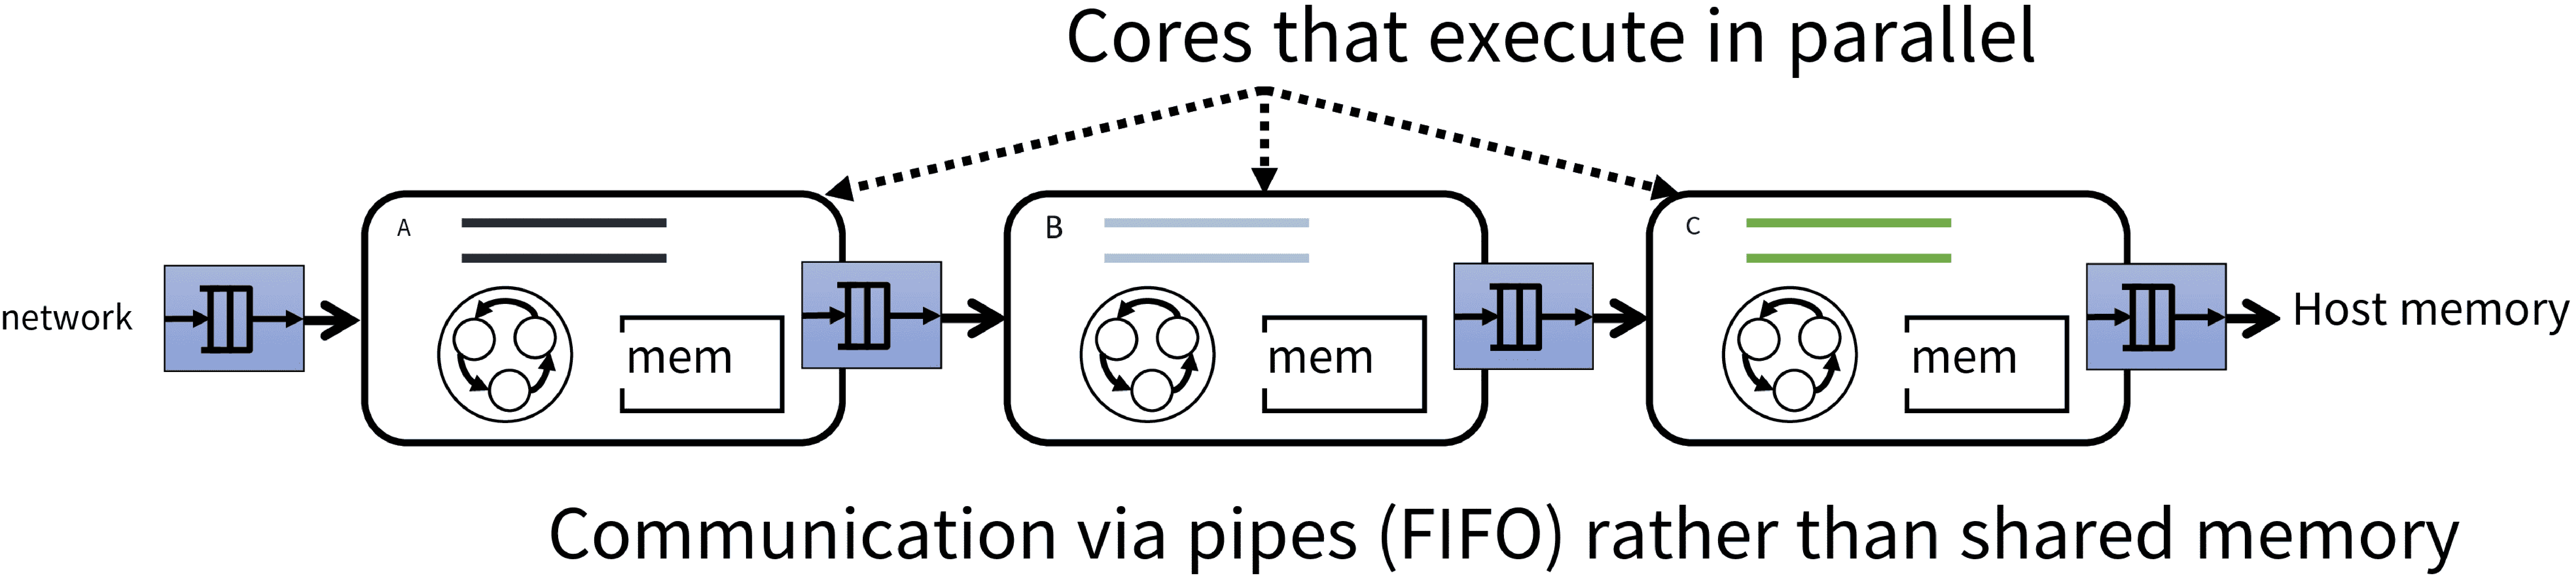
\includegraphics[width=1.0\textwidth]{image/element_conn.pdf}
	\caption{ClickNP 核之间以及核与网络、主机的通信方式:管道(FIFO)。}
	\label{intro:fig:element_conn}
\end{figure}


下文将介绍 \name{},一种新颖的FPGA加速网络功能平台,满足灵活性、模块化、高性能、低延迟和 CPU/FPGA 联合处理的要求。

\egg{
Today's data centers rely on a wide range of network functions to implement network virtualization, ensure security (e.g. firewalls and intrusion detection/prevention systems), perform measurements and improve performance (e.g. traffic scheduling). As data centers are moving towards 40 Gbps bandwidth at end hosts, where the line-rate is 60 M packets per second for minimum-sized packets, higher throughput requirement is imposed upon network processors. Furthermore, as data center services are evolving rapidly, programmability becomes indispensable for network processors. However, existing network processors has a large mismatch to the performance and programmability requirements.

\subsection{Architectures for Network Processors}

Network processors based on general-purpose CPUs such as ClickOS \cite{martins2014clickos} enjoy good programmablity, modularity and composabilty, but the packet forwarding performance of a single core could not keep up with 10 Gbps line rate for minimum-sized packets, even before any network function is plugged in. Because CPU instructions are executed one-by-one and have low parallelism, packet processing performance would drop further as more network functions are added. If a CPU-based network processor is added bump-in-the-wire, there will be 10s of microseconds additional end-to-end latency \cite{martins2014clickos} which is one magnitude higher than the switching fabric. In network virtualization scenario, if packet encapsulation and decapsulation is done at end hosts, as in the case of virtual switch, 网卡 offloading mechanisms including Large Send Offload (LSO) and Large Receive Offload (LRO) have to be disabled, which has a huge impact on TCP performance \cite{yoshino2008performance}.

ASICs are known to be high-performance, but the network functions are fixed. Commodity switching ASICs typically have a pipeline of network functions \cite{broadcomethernet}, where each function can be configured via registers and a match table based on TCAM or memory. Some ASICs provide flexible OpenFlow-like match-action tables \cite{broadcomopenflow}, but the packet parser is fixed (we could not support new packet header and shim layer formats), actions are not extensible and the order of network functions in the pipeline is not reconfigurable.

GPUs are widely used as co-processors for computing-intensive tasks, but its SIMD (Single-Instruction Multiple-Data) programming model does not fit network processing, where different types of packets may take various execution flows. The high power consumption, high latency of batch processing and inability to receive and send network packets without CPU intervention are also factors that render GPU-based network processor infeasible in data centers.

Fortunately, reconfigurable hardware is an architecture that provides both programmability, high performance and power efficiency for certain workloads. FPGA (field programmable gate arrays) is the most prominent example of reconfigurable hardware. FPGAs can implement arbitrary logic function and utilize distributed on-chip registers and SRAM to exploit bit-level and task-level parallelism, therefore stream processing pipelines would not ``hit the memory wall'' as in Von Neumann architecture \cite{bacon2013fpga}. FPGA has shown potential in accelerating many workloads in cloud \cite{putnam2014reconfigurable}. Moreover, Moore's law is still working in FPGA industry, because the fabrication technology of FPGA is currently several generations behind the CPU industry [citation required].

\subsection{FPGA Programming Challenge}

Despite FPGA's potential in network processing, the programmablity of FPGA is traditionally provided by hardware description languages (硬件描述语言) such as Verilog, which requires hardware knowledge and are much harder to program and debug than higher-level languages such as C/C++. Thus, existing FPGA-based network processors such as NetFPGA \cite{lockwood2007netfpga} are hard to program for software engineers.

Many works, e.g. OpenFlow \cite{mckeown2008openflow}, P4 \cite{bosshart2014p4} and 软件定义网络et \cite{xilinxsdnet}, provides the programmability by abstracting a set of primitives in network processing and defining a high-level programming language to compose the primitives. This direction has proved effective, but the programmability is limited to a set of pre-defined actions, which could not keep pace with rapid development of data center network functions. Our work strive to make the primitives extensible for software engineers.

Fortunately, several frameworks have been proposed to provide abstractions for generic FPGA programming. Examples of such works include Xilinx Vivado 高层次综合 (High Level Synthesis) \cite{feist2012vivado} based on C/C++, Altera SDK for OpenCL \cite{czajkowski2012opencl} based on C-like OpenCL and IBM Lime \cite{auerbach2010lime} based on Java.

However, FPGA has a completely different architecture than general-purpose CPUs. For software programmers that bear Von Neumann model in mind, the compilers may generate surprisingly poor hardware logic for reasonable code in high-level language. For example, Click2NetFPGA \cite{Click2NetFPGA} uses LLVM and 高层次综合 tools to compile optimized Click C++ code into 硬件描述语言, but the resulting FPGA-based router can only process 178 K pps (packets per second) for 98B packets, and 215 Mbps for large packets, which is 30 -- 50x slower than a CPU core in ClickOS \cite{martins2014clickos}. The bottleneck for small packets is the IP header checking stage \cite{Click2NetFPGA} because this stage is not fully pipelined; the bottleneck for large packets is the byte-wide shared memory \cite{Click2NetFPGA}, indicating a shared-memory design suitable for Von Neumann model would yield poor performance on FPGA.

FPGA has millions of logic gates with 10x slower clock rate than CPU, thousands of distributed fast SRAMs each with only KB capacity, and a large DRAM with 10x lower throughput than DRAMs in CPU architecture. Consequently, exploiting both spatial and temporal parallelism is crucial to unleashing the performance of FPGA. In network stream processing, most operations are independent of each other and therefore can be either parallelized (spatial) or pipelined (temporal), so that each stage of the pipeline can process different packets in parallel.

\subsection{Design Goals}
\label{clicknp:subsec:designgoals}

We highlight several design goals for our ClickNP framework to enable software engineers to write efficient network applications.

\smalltitle{Modularity.} Modularity is one key feature that improves parallelism, since modules do not have shared state and can run in parallel by nature. Borrowing the concepts from Click modular router \cite{kohler2000click}, \textit{elements} are basic building blocks of network functions. Elements run asynchronously and are connected via uni-directional \textit{channels}. The network processing pipeline is a data flow graph of elements and channels, starting from Ethernet receivers and ending at Ethernet transmitters.

\smalltitle{Line-rate throughput.} To allow efficient processing of packet content, an Ethernet packet is split into 32-byte \textit{flits} before feeding into elements. In the worst case, when 69-byte packets are received back-to-back, the line rate would be 40G / 8 / (69+20) = 56.18 Mpps, which splits into 56.18M * 3 = 168.54M flits. Every clock cycle an element reads at most one flit and outputs zero or one flit. This means any FPGA pipeline with clock frequency lower than 168.54 MHz would not be able to achieve line rate. If we waste a cycle between every two packets, the minimum clock frequency would be 224.72 MHz. However, on Stratix V FPGA platform \cite{stratix2012device}, non-trivial hardware logic that accesses registers and local memory can hardly run higher than 200 MHz. Therefore no idle cycles are allowed in elements processing packet content. First, the framework should provide abstractions for programmers to develop fully pipelined network functions. Second, as full compilation of a FPGA program may take hours, the framework should give performance warnings in an early compilation stage if the code cannot be fully pipelined.

\smalltitle{Code reuse.} Many network applications share a common set of elements, for example packet parser, lookup tables and packet modifications. Code of these elements should be reusable and elements should be composable. Software engineers should be able to write many network applications simply by connecting elements in the library.

\smalltitle{Debugging support.} First, as 硬件描述语言 (e.g. Verilog) simulation and debugging is both time consuming and requires extensive hardware knowledge, the framework should be able to compile OpenCL-based ClickNP programs to native x86 code for emulation, and provide traffic generators and receivers to test functionality. Second, as CPU is neither capable of sending or receiving packets at 60 Mpps, we need a FPGA-based network benchmark suite to perform stress testing on the network processor.

\smalltitle{Separation of control plane and data plane.} On one hand, our throughput requirement requires most network packets to be processed through the reconfigurable hardware without any CPU intervention. On the other hand, 软件定义网络 and 网络功能虚拟化 applications are usually complicated and have external dependencies. Therefore a clear interface between the control plane and the data plane is mandatory, where data plane programs are written within ClickNP framework and target massive parallelism, and control plane programs need only slight modifications to call our host library and perform on-the-fly reconfigurations.

\smalltitle{Host communication.} Network processors require low-latency and high-throughput interactions with the host machine. In 软件定义网络 and 网络功能虚拟化 applications, FPGA needs to send unknown packets to the controller and request a new forwarding rule to be inserted into FPGA. The round-trip time should be as low as possible to reduce end-to-end flow establish time. In packet replay and capture applications, FPGA needs to receive or send Gigabytes of packets from or to the host machine without using the network adapter.

We design ClickNP to meet the above design goals with Catapult FPGA \cite{putnam2014reconfigurable} and Altera OpenCL \cite{singh2011implementing}. In the next section, we will describe the FPGA and OpenCL components, and how we build a toolchain that abstracts away hardware specific details.
}

\egg{
\subsection{FPGA in datacenter}

Conventionally, datacenter operators largely relied on the performance improvements in general-purpose servers
to improve the operation efficiency. This performance improvement rate of servers 
has considerably slowed down recently due to the power limitations~\cite{putnam2014reconfigurable, more-citation}.
This has motivated the adoption of \textit{accelerator} that can be specialized to certain workloads to get efficiency gains.
However, the non-programmable ASIC-based accelerators are undesirable for datacenters due to following two reasons:
Firstly, datacenter operators prefers homogeneous server configurations to minimize the management overhead and also provide
a consistent platform that applications can rely on.
Secondly, services in datacenters evolve extremely rapidly. Waiting for the long release cycle of ASIC chips is undesirable.
%
Therefore, it requires a flexible accelerator that can potentially speed up many applications.
%
GPU and FPGA are two predominate technologies that satisfy this requirement.

% comparison between GPU and FPGA
% power efficiency
Compared with GPU, FPGA is more power efficient. For example, the latest NIVDIA xxx consumes xxx W power, while a high-end
Altera Stratix V consumes xxx W power ( J per op?) \knote{need a citation}. 
% versatile 
Further, FPGA is more versatile. While GPU is mainly designed to achieve \textit{data parallelism} with SPMD (single program, multiple data), 
FPGA can easily achieve both data parallelism and \textit{task parallelism} as different block of LEs can be independently configured to
implement different processing.  
% I/O
Finally, FPGA supports various I/O interface. Normally, GPU can only communicate with PC memory through PCIE bus. 
But FPGA can input or output data from many interfaces like network ports, and is more suitable for processing these 
I/O streams. 

FPGA is a mature technology and becomes inexpensive. A large scale deployment of FPGA in Microsoft datacenter shows 
that a high-end FPGA board increases the total cost of ownership (TCO) of a server by less than 30\%, but can double 
the Bing search efficiency~\cite{putnam2014reconfigurable}.
%
In this paper, we focus on using FPGA to accelerate network functions that are essential to our datacenter networks.
}

\egg{
\smalltitle{inexpensive}

Why I need this as background:
\begin{itemize}
\item Price issue?
\item Power?
\item Transition to FPGA for network functions?
\end{itemize}
}
